\begin{figure}
  \centering
    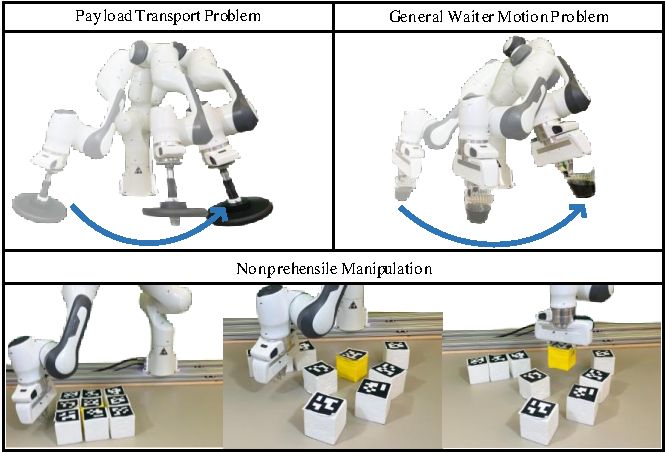
\includegraphics[width=\columnwidth,height=0.7\columnwidth]{assets/first_pg_final.pdf}
  \caption{Several applications motivate the need for considering dynamic constraints in motion planning. The payload transport problem requires the robot to account for the added mass at its end-effector and its effects on the inertia, Coriolis, and gravity matrices in the robot dynamics model \cite{saramago2002optimum}. Similarly, liquid transport in the General Waiter Motion Problem imposes acceleration constraints on the end-effector to ensure spill-free trajectories \cite{ichnowski2022gomp}. Nonprehensile actions like poking can be used to singulate target objects and require an understanding of combined robot and object dynamics \cite{pasricha2022pokerrt}. In this paper, we present a method for planning robot paths while considering its dynamic constraints.\vspace{-8pt}}\label{fig:first-page}
\end{figure}